\fancyhead[L]{}
\fancyhead[R]{\textsf{\textbf{MỤC 1.1}}\quad \textsf{Bốn cách biểu diễn một hàm số}\qquad \textbf{\textsf{17}}}

\noindent
\begin{minipage}[t]{0.26\textwidth}
    \vspace*{3.6cm}
    \raggedleft
    \textbf{\textsf{HÌNH 22}}

    \vspace{1.1cm}
    \centering
    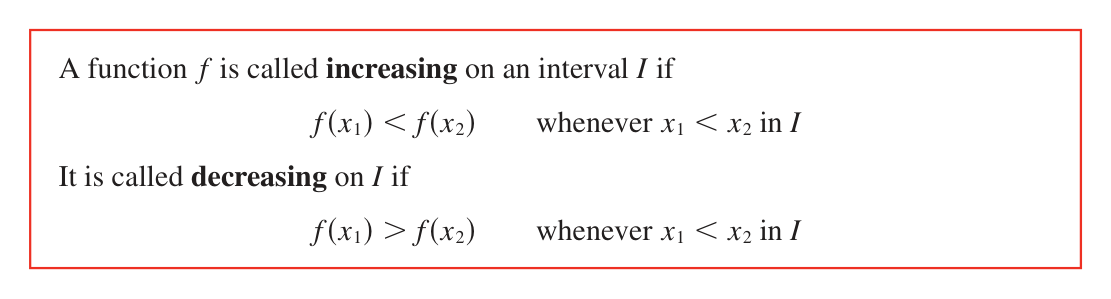
\includegraphics[width=0.95\linewidth]{images/p0052_fig2.png}
    
    \vspace{0.1cm}
    \raggedright
    \textbf{\textsf{HÌNH 23}}
\end{minipage}%
\hfill
\begin{minipage}[t]{0.71\textwidth}
    \noindent
    $a$ và $b$ với $x_1 < x_2$, thì $f(x_1) < f(x_2)$. Chúng ta dùng điều này làm tính chất định nghĩa của một hàm số đồng biến.

    \vspace{0.15cm}
    \centering
    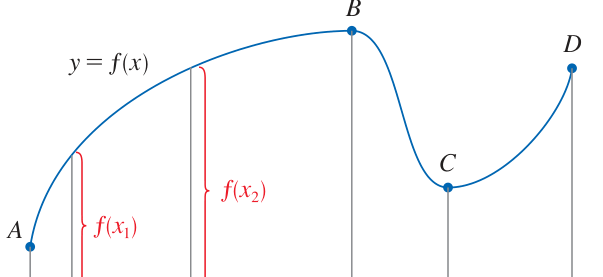
\includegraphics[width=0.98\linewidth]{images/p0052_fig1.png}

    \vspace{0.2cm}
    \raggedright
    \begin{definitionbox}
        Một hàm số $f$ được gọi là \textbf{đồng biến} trên một khoảng $I$ nếu
        \[
        f(x_1) < f(x_2) \quad \text{mỗi khi } x_1 < x_2 \text{ trong } I
        \]
        Nó được gọi là \textbf{nghịch biến} trên $I$ nếu
        \[
        f(x_1) > f(x_2) \quad \text{mỗi khi } x_1 < x_2 \text{ trong } I
        \]
    \end{definitionbox}

    \vspace{0.15cm}
    \noindent
    Trong định nghĩa của hàm số đồng biến, điều quan trọng cần nhận ra là bất đẳng thức $f(x_1) < f(x_2)$ phải được thỏa mãn đối với \emph{mọi} cặp số $x_1$ và $x_2$ trong $I$ với $x_1 < x_2$.

    \noindent
    Bạn có thể thấy từ Hình 23 rằng hàm số $f(x) = x^2$ nghịch biến trên khoảng $(-\infty, 0]$ và đồng biến trên khoảng $[0, \infty)$.
\end{minipage}

\vspace{0.35cm}
\noindent
{\color{stewartcyan}\rule{\linewidth}{1.2pt}}\\[-0.65em]
{\color{stewartcyan}\rule{\linewidth}{0.6pt}}

\vspace{0.15cm}
\noindent
{\Large\textbf{\textsf{\color{stewartcyan}1.1}}\quad {\color{stewartcyan}\rule[-2pt]{1.5pt}{13pt}}\quad \textbf{\textsf{BÀI TẬP}}}

\vspace{0.25cm}
\noindent
\begin{minipage}[t]{0.485\textwidth}
    \textbf{1.} Nếu $f(x) = x + \sqrt{2 - x}$ và $g(u) = u + \sqrt{2 - u}$, có đúng khi nói $f = g$ không?

    \vspace{0.2cm}
    \textbf{2.} Nếu
    \[
    f(x) = \frac{x^2 - x}{x - 1} \quad \text{và} \quad g(x) = x
    \]
    có đúng khi nói $f = g$ không?

    \vspace{0.2cm}
    \textbf{3.} Đồ thị của một hàm số $g$ được cho như hình bên.
    \begin{enumerate}[label=(\alph*), leftmargin=*, itemsep=0pt, topsep=1pt, parsep=0pt]
        \item Nêu các giá trị của $g(-2)$, $g(0)$, $g(2)$ và $g(3)$.
        \item Với (những) giá trị nào của $x$ thì $g(x) = 3$?
        \item Với (những) giá trị nào của $x$ thì $g(x) \leqslant 3$?
        \item Nêu tập xác định và tập giá trị của $g$.
        \item Trên (những) khoảng nào thì $g$ đồng biến?
    \end{enumerate}

    \vspace{0.15cm}
    \centering
    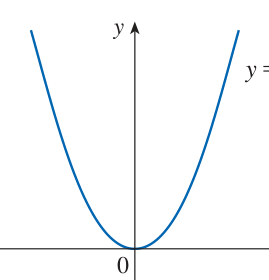
\includegraphics[width=0.72\linewidth]{images/p0052_fig3.png}
\end{minipage}%
\hfill
\begin{minipage}[t]{0.485\textwidth}
    \textbf{4.} Đồ thị của $f$ và $g$ được cho như hình bên.
    \begin{enumerate}[label=(\alph*), leftmargin=*, itemsep=0pt, topsep=1pt, parsep=0pt]
        \item Nêu các giá trị của $f(-4)$ và $g(3)$.
        \item Giá trị nào lớn hơn, $f(-3)$ hay $g(-3)$?
        \item Với những giá trị nào của $x$ thì $f(x) = g(x)$?
        \item Trên (những) khoảng nào thì $f(x) \leqslant g(x)$?
        \item Nêu nghiệm của phương trình $f(x) = -1$.
        \item Trên (những) khoảng nào thì $g$ nghịch biến?
        \item Nêu tập xác định và tập giá trị của $f$.
        \item Nêu tập xác định và tập giá trị của $g$.
    \end{enumerate}

    \vspace{0.15cm}
    \centering
    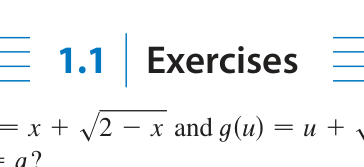
\includegraphics[width=0.72\linewidth]{images/p0052_fig4.png}

    \vspace{0.25cm}
    \raggedright
    \textbf{5.} Hình 1 được ghi lại bởi một thiết bị do Sở Mỏ và Địa chất California vận hành tại
\end{minipage}